%Context
\chapter{背景介绍}
\label{sec-context} %Label for cross-referencing

\section{需求陈述}
\label{sec:need}

整体目标:

我们旨在设计出一种实时的远程音视频通信,将两处的信息交流接合,这种设计
基于一台有灵敏移动性能且具备基础的环境障碍感知能力的移动机器人。

背景及意义:

随着计算机、互联网技术的飞速发展,人与人、人与事物之间的联系日益密切,
人们所接触的范围也逐渐广泛起来,于此同时,所需要的信息流量也会大大增加,
传统的传递方式也许并不能很好的起到传递效果。如果让数字化介入其中,便会
收获更好的结果。

试想一下,当某一个机构或部门需要向外界介绍他们的相关信息,这些信息会给
参观者留下非常重要的印象,如果诸如此类的信息能够具有实时性、全方位性,
并且能够充分调动参观者的主观感受,那么这些信息的价值便会大大提升。

通过远程呈现的基本构架,借助移动机器人提供的主观能动性,搭建如此的一个
集散控制的参观导航系统,便会具有如上所述的极佳的效果。

当你身处千里之外,通过简单的互联网界面,点击鼠标、敲击键盘,就可以达到
参观目的地的效果,而且这种信息的获取是实时动态的,该是一件多么惬意的事
情,你一定会对目标地点有一个非常好的主观印象。而且,你还可以随时与那里
的工作人员等互动交流,岂不是更加便捷、实用!

\section{问题陈述}
\label{sec:problem}

进一步分析目标,我们可以将过程中需要着重注意、解决的难题归纳总结,分成
不同的项目部分,以备后续逐步实现预订功能。如下为分类:

\begin{itemize} \tightlist
\item 网络连接搭建的方式

\item 远程操作者的使用界面

\item 机器人上的用户界面

\item 机器人的操控方式

\end{itemize}

对于网络搭建,由于机器人可能部署在任意的网络环境中,因此不能对实现这套
系统的网络有过高的要求与假设。我们的设计目标是部署在机器人上的客户端无
需公网地址段的ip,也无需和使用者处于同一个子网内,只要机器人有一个无线
网络连接,就可以正常工作。

对于使用界面的设定,考虑到跨平台的潜在需求和移动互联网的趋势,应该采用
基于网页界面的设计,具体的功能模块后续的设计中会逐渐添加,进而集成到界
面中,以达到符合用户使用需求的目标。

机器人的控制方式也是一个非常重要的方面,它直接关系到了机器人的安全性等
强制性的因素,而且对于用户体验也是至关重要的。

\section{组员介绍}
\label{sec:team}

\begin{framed}
\noindent 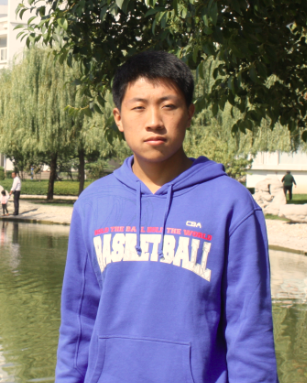
\includegraphics[width=50mm]{Figures/context.pic.png}
\parbox[b]{0.6\textwidth}{王照栋\\
现况:中国科学技术大学,自动化系,10级本科生\\
邮件:wangzd@mail.ustc.edu.cn\\
技能:基础机械结构设计,自动控制\\
编程:C语言编程,初步C++面向对象编程,matlab\\
}

来自山东,2010年考入中科大信息学院,后就读于自动化系。喜欢设计,并且具
有一定的动手能力,2012年暑期与同学组队参加过Robogame机器人大赛,并最终
获最佳技术奖单项奖。课余时间比较喜欢参与一些运动以及益智类的活动,热爱
乒乓球、篮球、羽毛球、游泳等运动,对魔方速拧还原有一定的研究。
\end{framed}

\begin{framed}
\noindent
%\parbox[b]{0.6\textwidth}
{贾肇聪\\
现况:中国科学技术大学10级少年班学院\\
}
自由软件爱好者,在本项目中负责linux服务器的管理和网络维护。
\end{framed}
